\documentclass[a4paper, 14pt]{extarticle}

\usepackage[T2A]{fontenc}
\usepackage{natbib}
\usepackage{graphicx}
\usepackage[english, russian]{babel}
\usepackage{fontspec}
\usepackage{amsmath}
\usepackage{amsfonts}
\usepackage{amssymb}
\usepackage{amsthm}
\usepackage{mathtools}
\usepackage{mathrsfs}
\usepackage{icomma}
\usepackage{fullpage}
\usepackage{ulem}
\usepackage{setspace}
\usepackage{listings}
\usepackage{indentfirst}
\usepackage[left=2cm,right=1.5cm,top=2cm,bottom=2cm]{geometry}
\usepackage{xcolor}
\usepackage{float}
\usepackage{csquotes}
\usepackage{hyperref}
\usepackage{graphics}



\definecolor{urlcolor}{HTML}{0000FF} % цвет гиперссылок
\definecolor{linkcolor}{HTML}{000000} % цвет гиперссылок
\hypersetup{pdfstartview=FitH, linkcolor=linkcolor, urlcolor=urlcolor, colorlinks=true}


\setmainfont{Times New Roman}
\setlength{\parindent}{5ex}
\setlength{\parskip}{1em}
\renewcommand{\baselinestretch}{1}

\graphicspath{{images/}}


\definecolor{buzzlightyear}{HTML}{8757A5}
\definecolor{grass}{HTML}{738D06}
\definecolor{literal}{HTML}{F18A2B}
\definecolor{commentcolor}{HTML}{8E908B}

\lstdefinestyle{habrstyle}{
    backgroundcolor=\color{white},
    commentstyle=\color{commentcolor},
    keywordstyle=\bfseries\color{buzzlightyear},
    numberstyle=\tiny\color{commentcolor},
    stringstyle=\color{grass},
    basicstyle=\ttfamily\footnotesize,
    breakatwhitespace=false,
    breaklines=true,
    captionpos=b,
    keepspaces=true,
    numbers=left,
    numbersep=5pt,
    showspaces=false,
    showstringspaces=false,
    showtabs=false,
    tabsize=4
}

\lstset{style=habrstyle}

\begin{document}
    % НАЧАЛО ТИТУЛЬНОГО ЛИСТА
    \begin{center}
        \begin{center}
            \hfill \break
            \normalsize{Санкт-Петербургский государственный политехнический}\\
            \normalsize{университет Петра Великого}\\
            \hfill \break
            \normalsize{\textbf{Высшая школа интеллектуальных систем и}}\\
            \normalsize{\textbf{суперкомпьютерных технологий}}\\
            \hfill \break
            \hfill \break
            \hfill \break
            \normalsize{Лабораторная работа}\\
            \hfill \break
            \normalsize{\LARGE Дискретное преобразование Фурье}\\
        \end{center}
        \hfill \break
        \hfill \break
        \hfill \break
        \hfill \break
        \hfill \break
        \hfill \break
        \hfill \break
        \hfill \break
        \hfill \break
        \hfill \break
        \begin{tabbing}
            Выполнил студент гр. 3530901/80201 \`И.С. Иванов\\
            \\
            Преподаватель: \`Н.В. Богач\\
        \end{tabbing}
        \hfill \break
        \hfill \break
        \hfill \break
        \hfill \break
        \begin{center}
            Санкт-Петербург\\
            2021
        \end{center}
        \thispagestyle{empty}
    \end{center}
    % КОНЕЦ ТИТУЛЬНОГО ЛИСТА

    % ОГЛАВЛЕНИЕ
    \newpage
    \tableofcontents

    % СПИСОК ИЛЛЮСТРАЦИЙ
    \newpage
    \listoffigures

    % СПИСОК ЛИСТИНГОВ
    \newpage
    \lstlistoflistings

    \newpage


    \section{Упражнение №1}
    \label{sec:1}

    В первом упражнении необходимо просмотреть все примеры из файла \texttt{chap07.ipynb}.
    В этом файле приводятся примеры работы с сложными синусоидальными сигналами и примеры работы ДПФ.

    Все примеры запустились и были изучены.

    \begin{figure}[H]
        \centering
        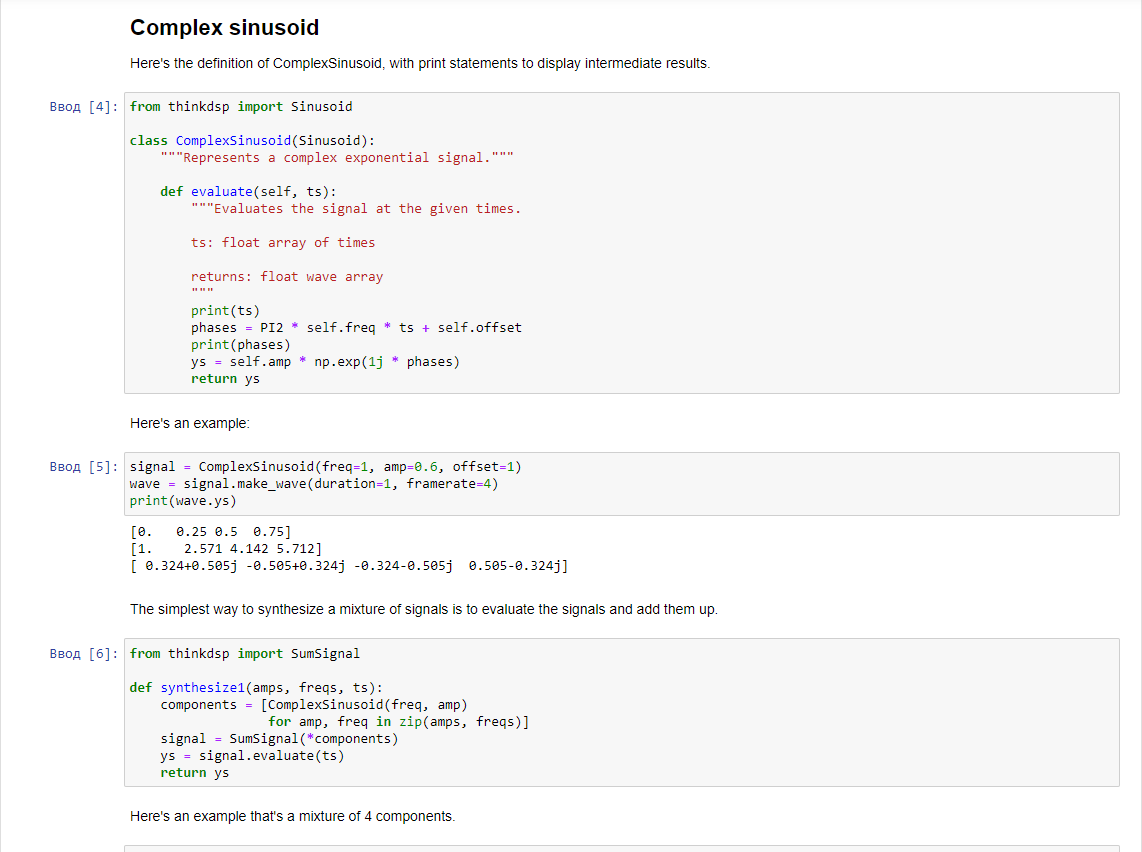
\includegraphics[width=0.8\linewidth]{check_work}
        \caption{Запуск примеров}
        \label{fig:check_work}
    \end{figure}

    \newpage


    \section{Упражнение №2}
    \label{sec:2}

    Во втором пункте седьмой лабораторной работы было продемонстрировано использование ДПФ (дискретное преобразование Фурье) и обратное ДПФ в виде произведения матриц.
    Такие операции занимают время \texttt{\(Nˆ2\)}, где \texttt{N} - длина массива, что достаточно быстро для большинства применений, но есть более быстрый алгоритм.
    Быстрое Преобразование Фурье (БПФ) или \texttt{FFT}, занимающий \texttt{\(Nlog(N)\)}.
    Ключевая вещь в БПФ это лемма Даниелсона-Ланцоша, которая предлагает рекурсивный алгоритм для DFT:
    \begin{enumerate}
        \item Входящий массив \texttt{y} разделяется на четное число элементов \texttt{e}, и на нечётные элементы \texttt{o}.
        \item Вычислить \texttt{DFT} \texttt{e} и \texttt{o} с помощью рекурсивных запросов.
        \item Вычислить \texttt{DFT(y)} для каждого значения \texttt{n} используя лемму Даниелсона-Ланцоша.
    \end{enumerate}
    В случае если длина исходного массива равна 1, \texttt{DFT(y) = y}.
    Или если длина y очень мала, можно вычислить её \texttt{DFT} с помощью матричного умножения, используя предварительно вычисленную матрицу.

    Начнем с реального сигнала и вычислим его БПФ.

    \begin{lstlisting}[language=Python, caption= Получение БПФ, label={lst:get_bpf}]
        ys = [-0.5, 0.1, 0.7, -0.1]
        hs = np.fft.fft(ys)
        print(hs)
    \end{lstlisting}

    Получившиеся значения: \texttt{[ 0.2+0.j -1.2-0.2j 0.2+0.j -1.2+0.2j]}

    Реализуем функцию \texttt{dft} для вычисления матрицы синтеза и протестируем ее.

    \begin{lstlisting}[language=Python, caption= Функция dft, label={lst:dft}]
        def dft(ys):
            N = len(ys)
            ts = np.arange(N) / N
            freqs = np.arange(N)
            args = np.outer(ts, freqs)
            M = np.exp(1j * PI2 * args)
            amps = M.conj().transpose().dot(ys)
            return amps
    \end{lstlisting}

    \begin{lstlisting}[language=Python, caption= Использование dft, label={lst:call_dft}]
        hs2 = dft(ys)
        np.sum(np.abs(hs - hs2))
    \end{lstlisting}

    Получившиеся значение 5.864775846765962e-16.

    Реализуем функцию \texttt{fft\_norec}, которая разобьет входной массив и использует \texttt{np.fft.fft} для вычислеия БПФ.

    \begin{lstlisting}[language=Python, caption= Функция fft\_norec, label={lst:fft_norec}]
        def fft_norec(ys):
            N = len(ys)
            He = np.fft.fft(ys[::2])
            Ho = np.fft.fft(ys[1::2])

            ns = np.arange(N)
            W = np.exp(-1j * PI2 * ns / N)

            return np.tile(He, 2) + W * np.tile(Ho, 2)
    \end{lstlisting}

    \begin{lstlisting}[language=Python, caption= Использование fft\_norec, label={lst:call_fft_norec}]
        hs3 = fft_norec(ys)
        np.sum(np.abs(hs - hs3))
    \end{lstlisting}

    Получившиеся значение 0.0.

    Реализуем функцию \texttt{fft}.
    Она похожа на предыдущую, но в ней \texttt{np.fft.fft} заменено на рекурсию.

    \begin{lstlisting}[language=Python, caption= Функция fft, label={lst:fft}]
        def fft(ys):
            N = len(ys)
            if N == 1:
                return ys

            He = fft(ys[::2])
            Ho = fft(ys[1::2])

            ns = np.arange(N)
            W = np.exp(-1j * PI2 * ns / N)

            return np.tile(He, 2) + W * np.tile(Ho, 2)
    \end{lstlisting}

    \begin{lstlisting}[language=Python, caption= Использование fft, label={lst:call_fft}]
        hs4 = fft(ys)
        np.sum(np.abs(hs - hs4))
    \end{lstlisting}

    Получившиеся значение 1.6653345369377348e-16.

    В результате можно сказать, что полученная нами реализация БПФ занимает время, пропорциональное \texttt{\(Nlog(N)\)} при создании и копировании массивов, а также занимает аналогичное количество места.

    \newpage


    \section{Выводы}
    \label{sec:conclusions}

    В результате выполнения данной лабораторной работы были изучены понятия ДПФ, БПФ.
    Была создана функция для вычисления БПФ, которая работает за \texttt{\(Nlog(N)\)} при создании и копировании массивов.
    Кроме того мы изучили примеры из файла \texttt{chap07.ipynb}, запустив все блоки кода и прочитав всю информацию.

\end{document}